\section{Results}

We have analysed more than 400 dependent variables. In this section we report the results for variables which showed a statistically significant difference between the B and HT conditions. The full table is provided as a supplementary material. 
The variables are divided in five groups: movement of the head in space, users' performance and self-assessment, joint moments, muscle forces, and muscle activation.

\subsection{Movement of the head}

% code in file QuestionnaireAnalysis-RProj/analyse_head_movement2.R

\begin{figure}[tb]
\centering%
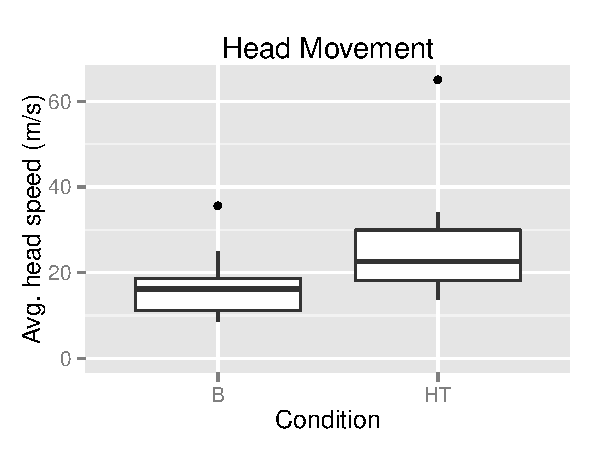
\includegraphics[width=\columnwidth]{img/HeadMovement-ggplot}%
\caption{Subjects' head average speed in the two conditions.}%
\label{fig:head-movement}
\end{figure}

This section describes how we verified that the parallax effect effectively induced the subjects to increase the movement of their head. We considered the the motion of the head as captured by the motion capture system. More precisely, we extracted the x, y, z motion coordinates of the marker positioned over the right eye. For each user, and separately for the B and HT conditions, we integrated the traveled path and normalized it by the time spent in accomplishing the task. The result is the average speed of the head during a task in a given condition.

Between trials, subjects were often observed to sit back on the chair in order to relax or discuss with the operator. In so doing, they were performing wide head movements which were not functional to the accomplishment of the task.
Hence, the motion has been considered only for the time spent between the actual beginning of a trial, when the user first pinched the object, and its accomplishment, when the user performed the last drop in the target container.
The measured head average speed is 16.21 m/s (SD=5.95) for the B condition and 24.51 m/s (SD=9.89) for the HT condition (see Figure \ref{fig:head-movement}).

A Shapiro-Wilk normality test showed that the distribution of speeds in the B condition is normal (p=0.0117), but not for the HT condition (p~\textless~0.001). Hence we measure the statistical difference in the two conditions using a Wilcoxon signed rank test. Results show a statistically significant difference in the average speed in the two conditions (V=23, p~\textless~0.001).
We can hence hence assume with 99.9\% confidence that the parallax effect indeed invited the users to perform head movements on average 51.17\% wider than without tracking.


\subsection{User performance and subjective measures}


% questionnarie
After the experiment, subjects were asked to fill a questionnaire to self-assess how much they liked the interface and how much pain in the shoulder they felt after the first and after the second task.

% liked the interface?
% QuestionnaireAnalysis-RProj/analyse_F.R
% QuestionnaireAnalysis-RProj/analyse_C.R
Twenty-three out of the thirty subjects answered the question: ``How did you find the interaction overall?", on a scale from 1 (bad) to 6 (good). The results reported in the following table (M=4.48, SD=0.89).

%appreciation
% 1  2  3  4  5  6 
% 0  1  1  9 10  2 

\begin{center}
\begin{tabular}{ | c | c | c | c | c | c | c | }
\hline
& bad & \ldots  & \ldots & \ldots & \ldots & good \\
\hline
Vote & 1 & 2 & 3 & 4 & 5 & 6 \\
\hline
Count & 0 & 1 & 1 & 9 & 10 & 2 \\
\hline
\end{tabular}\end{center}

Twenty-height out of the thirty subjects answered Yes or No on the question: ``Did you find useful the camera movement?''. Nineteen subjects (67.86\%) answered Yes.
Together with the previous results it indicates an overall good appreciation of the interaction method.

% QuestionnaireAnalysis-RProj/analyse_performance.R
% Performance (avg observation duration==docking time)
Subjects performed an average of 63.97 docking operations (SD=21.53) in the B condition and an average of 68.07 (SD=22.47) in the HT condition.
In terms of average time needed to accomplish a docking trial, the results are 12.72 secs (SD=8.45) for the B condition and 11.66 seconds (SD=5.54) for the HT condition.
% t.test w/ respect to conditions
A paired Wilcoxon signed rank test shows that there is no significant difference between the average time needed by a user to accomplish a docking trial between the B and the HT conditions (V=152, p=0.0998).


% Borg self-assessment for pain
% QuestionnaireAnalysis-RProj/analyse_borg.R
We observed that most of the subjects reported a slight pain in the shoulder already after the first condition. It is coherent with the self-assessment reported in the questionnaires.
Twenty-three out of the thirty subjects did a self-assessment of the pain perceived in their arm after the first and the second conditions, i.e., after 15 minutes and after 30 minutes. The assessment is based on the Borg RPE (Rate of Perceived Exertion) scale \cite{borg_borgs_1998}.
The Borg scale ask subjects to self-assess the perceived pain on a scale from 6 (no exertion at all) to 20 (maximal exertion).
After the first 15 minutes, subjects reported an average perceived pain of 11.93 points (min=6, max=19, SD=2.76). At the end of the second condition, after 30 minutes, the subjects reported an average of 11.34 points (min=6, max=16, SD=2.76).
In both conditions, the Borg scores follow a normal distribution. A paired t-test shows that there is no statistical difference in the perceived level of pain between the two conditions (t(22)=1.45, p=0.1622).
It means that the pain felt by the users has been provoked within the first 15 minutes of use of the interface, and the perceived pain remained stable until the 30th minute.


\subsection{Joint moments}

\begin{figure}[tb]
\centering%
%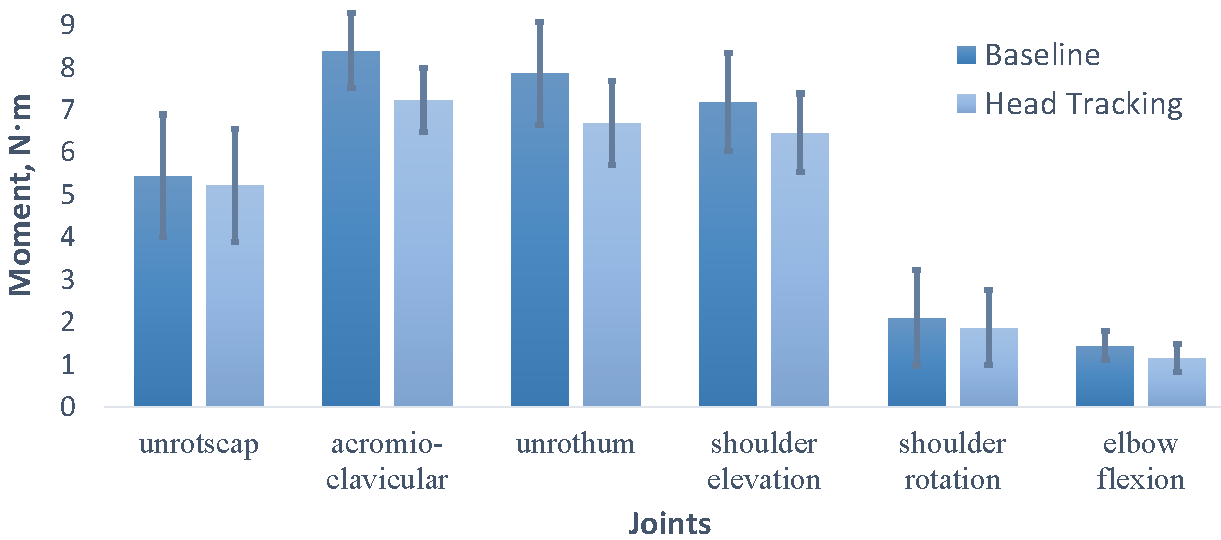
\includegraphics[width=\columnwidth]{img/ShoulderJointMoments1}%
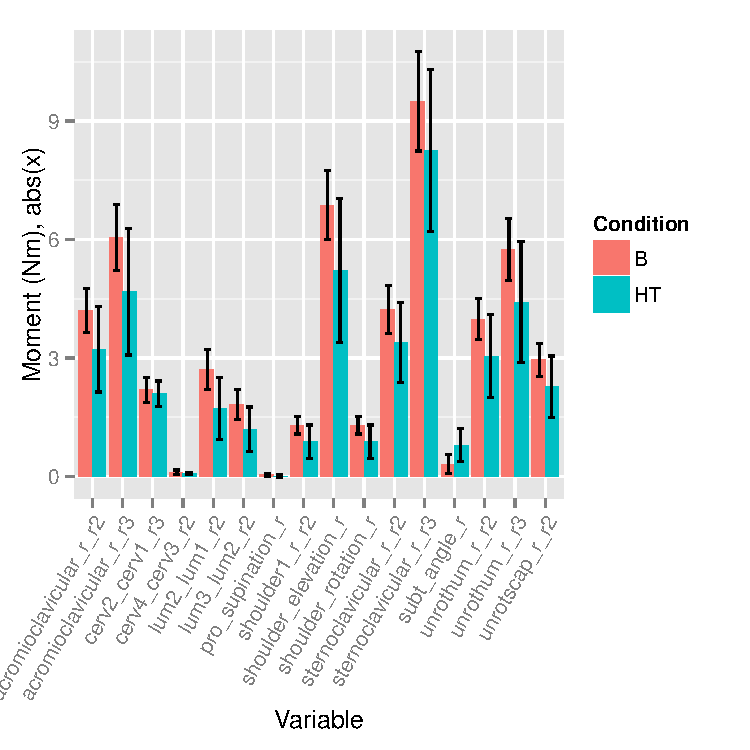
\includegraphics[width=\columnwidth]{img/Moments}%
\caption{The joints' degree of freedom whose moment magnitude changed significantly between B and HT conditions. Vertical bars denote 95\% confidence intervals.}%
\label{fig:moments}
\end{figure}

The moment magnitude (measure in Newton per meters) exerted at each joint has been measured with 103 variables. Each variable represent a degree of freedom of a joint. Each joint is modelled with one to three degrees of freedom.
A significant difference of the moments between B and HT conditions is present in 16 variables.
As can be observed in Figure~\ref{fig:moments}, the average magnitudes of 15 out 16 joint moments is decreased in head tracking condition comparing to the baseline by 4.2\%-19.9\% depending on a joint. There were significant differences for elbow flexion moment between HT (M=1.16, SD=1.37) and B (M=1.45, SD=0.59) conditions, t(29)=2.10, p=0.05; for sternoclavicular moment between HT (M=10.178, SD=3.86) and B (M=10.381, SD=3.56), t(29)=1.91, p=0.07. Unrotscapular, acromioclavicular, unrothumeral moments were less significant (0.1~\textless ~p~\textless~0.2) with differences between conditions 4.2\%, 13.8\% and 14.9\% respectively.

For unused upper extremity only slight increase in sternocalvicular moment is significant between HT (M=4.43, SD=2.95) and B (M=4.36, SD=2.57), t(29)=-1.69, p=0.1. The mean magnitudes of joint moments in lumbar and upper back and neck slightly decrease for most but 2 joints. The decreases in moments are significant for all neck joints (p~\textless~0.1), while the increases are not significant (0.2~\textless~p).
In the lower body there are significant increases by 8.1\% in hip moments t(29)=-1.76, p=0.09 and 22.7\% decrease in knee moments t(29)=1.89, p=0.07.



\subsection{Muscle forces}

\begin{figure}[tb]
\centering%
%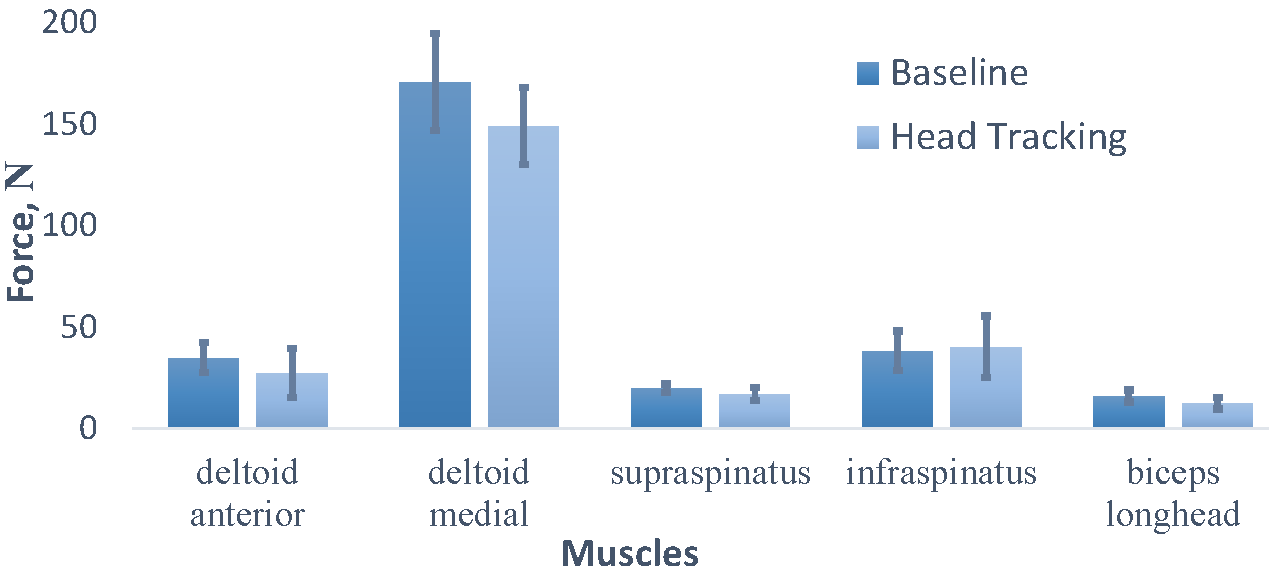
\includegraphics[width=\columnwidth]{img/MuscleForces}%
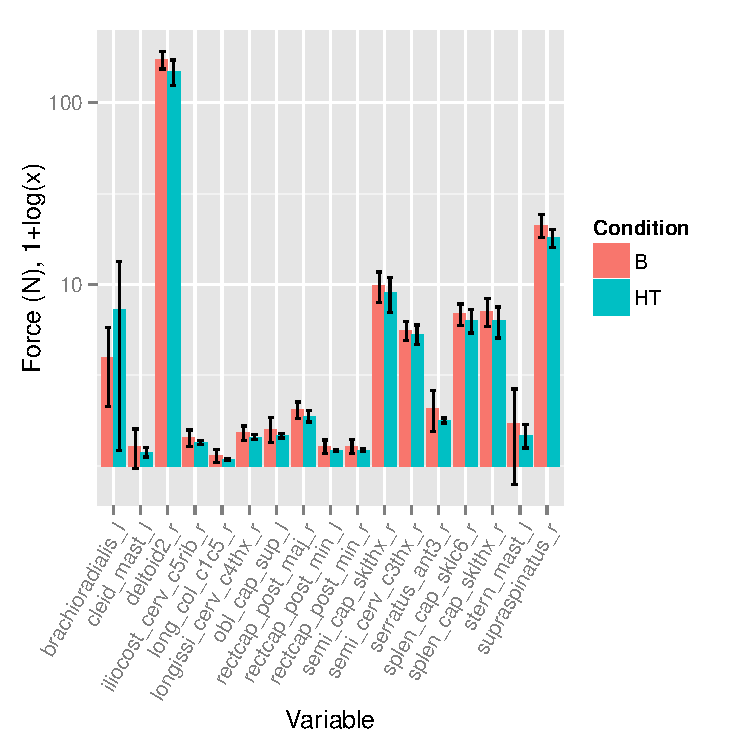
\includegraphics[width=\columnwidth]{img/Forces}%
\caption{The muscles whose exerted forces changed significantly between B and HT conditions. Vertical bars denote 95\% confidence intervals.}%
\label{fig:forces}
\end{figure}


As can be seen on Figures~\ref{fig:forces} and \ref{fig:activations}, muscle forces and activations demonstrate the same pattern in differences between the conditions.

\subsection{Muscle activations}

\begin{figure}[tb]
\centering%
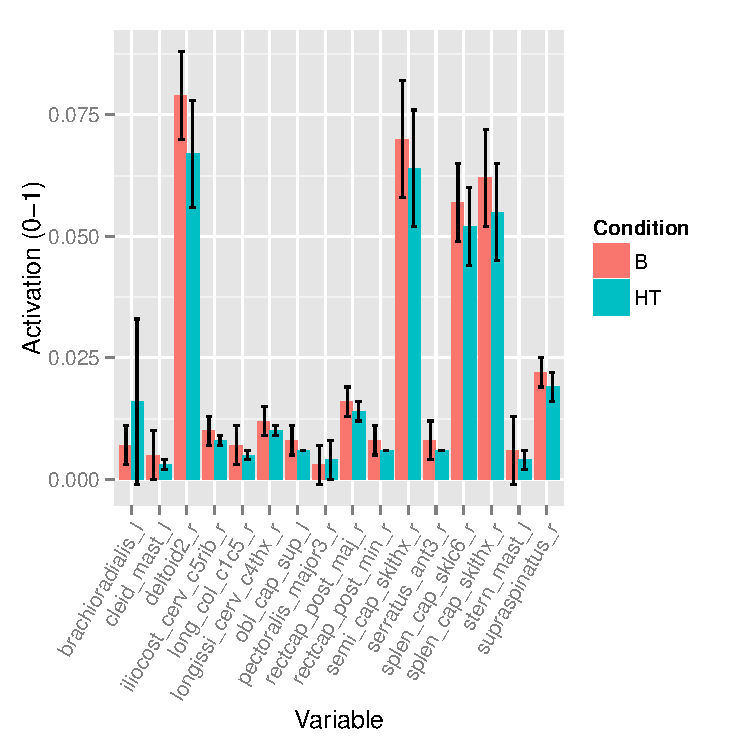
\includegraphics[width=\columnwidth]{img/Activations}%
\caption{
The muscles whose activation factor changed significantly between B and HT conditions. Vertical bars denote 95\% confidence intervals.}%
\label{fig:activations}
\end{figure}

 In the paper we provide values for the activations, as they roughly represent forces normalized by the size of each muscle and thus are considered on the same scale for all muscles. There are significant differences in activation of medial deltoid between HT (M=0.068, SD=0.031) and B (M=0.078, SD=0.025) conditions, t(29)=2.66, p=0.01; for supraspinatus: HT (M=0.019, SD=0.007) and B (M=0.022, SD=0.008), t(29)=2.05, p=0.05; and biceps longhead: HT (M=0.010, SD=0.006) and B (M=0.012, SD=0.006), t(29)=2.15, p=0.04. Less significant are differences for deltoid anterior: HT (M=0.012, SD=0.009) and B (M=0.015, SD=0.015), t(29)=1.52, p=0.14; for infraspinatus: HT (M=0.0164, SD=0.011) and B (M=0.0159, SD=0.016), t(29)=1.47, p=0.15; for brachioradialis: HT (M=0.009, SD=0.004) and B (M=0.010, SD=0.009), t(29)=1.38, p=0.18. To demonstrate the scale of the variable ``average activations'', the median for HT condition is 0.0055, and the median for the baseline is 0.0057.

There are no significant differences for muscle activations of lumbar region, but there are significant decreases by 7.3-15.7\% in activations of 2 upper back and neck muscles: splenius capitis and semispinalis capitis, (p~\textless~0.1). Multiple less recruited upper body muscles exhibit increase in their activation, however the increase is not significant.
